\begin{frame}
    \frametitle{AHTR Temperature Model}
    \begin{block}{AHTR Temperature Model}
        \begin{itemize}
            \item I used the open-source MSR simulation tool, Moltres, to conduct AHTR
            full assembly multiphysics simulations 
            \item AHTR Moltres simulations captures thermal feedback effects, absent
            from the purely neutronics OpenMC simulations
        \end{itemize}
    \end{block}

    \begin{block}{Steps to produce Moltres AHTR Temperature Model}
        \begin{itemize}
          \item OpenMC neutronics model produces group constants data for the Moltres model
          \item Moltres model mesh generation
          \item Moltres temperature model accepts group constants data and mesh
        \end{itemize}
    \end{block}

\end{frame}

\begin{frame}
    \frametitle{AHTR Temperature Model}
    \begin{block}{Energy Homogenization}
        \begin{table}[]
            \centering
            \begin{minipage}[c]{0.6\textwidth}
                \centering
                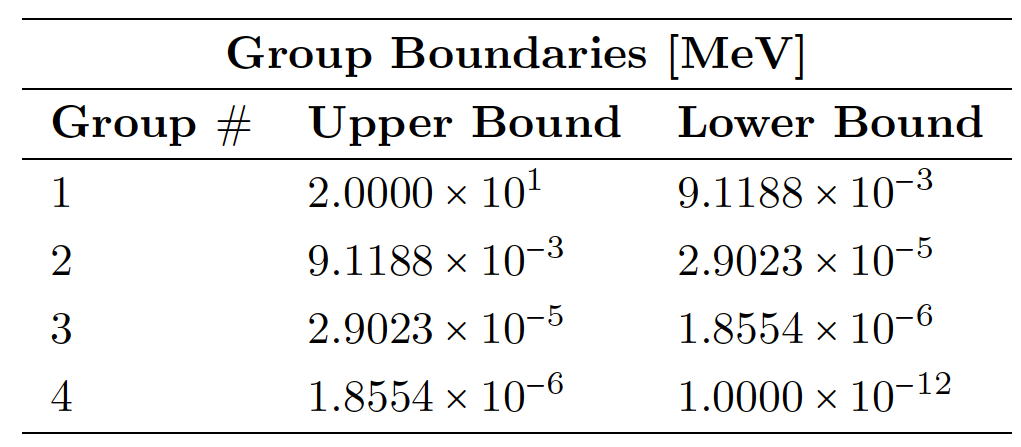
\includegraphics[width=0.8\linewidth]{figures/ahtr-energy-discr.png}
            \end{minipage}\hfill
            \begin{minipage}[c]{0.4\textwidth}
            \caption{4-group energy structures for AHTR geometry 
            derived by \cite{gentry_development_2016}.}
        \end{minipage}
        \end{table}
    \end{block}
\end{frame}

\begin{frame}
    \frametitle{AHTR Temperature Model}
    \begin{block}{Spatial Homogenization}
        Fuel slab discretization into 61 cells: inter-assembly FLiBe, Y-shaped graphite 
        structure, control rod slot FLiBe, graphite spacers, each diamond shape 
        section's inter-plank FLiBe (3), each graphite plank (18), and each
        fuel stripe (36)
    \end{block}
    \begin{figure}[]
        \begin{minipage}[c]{0.6\textwidth}
            \centering
            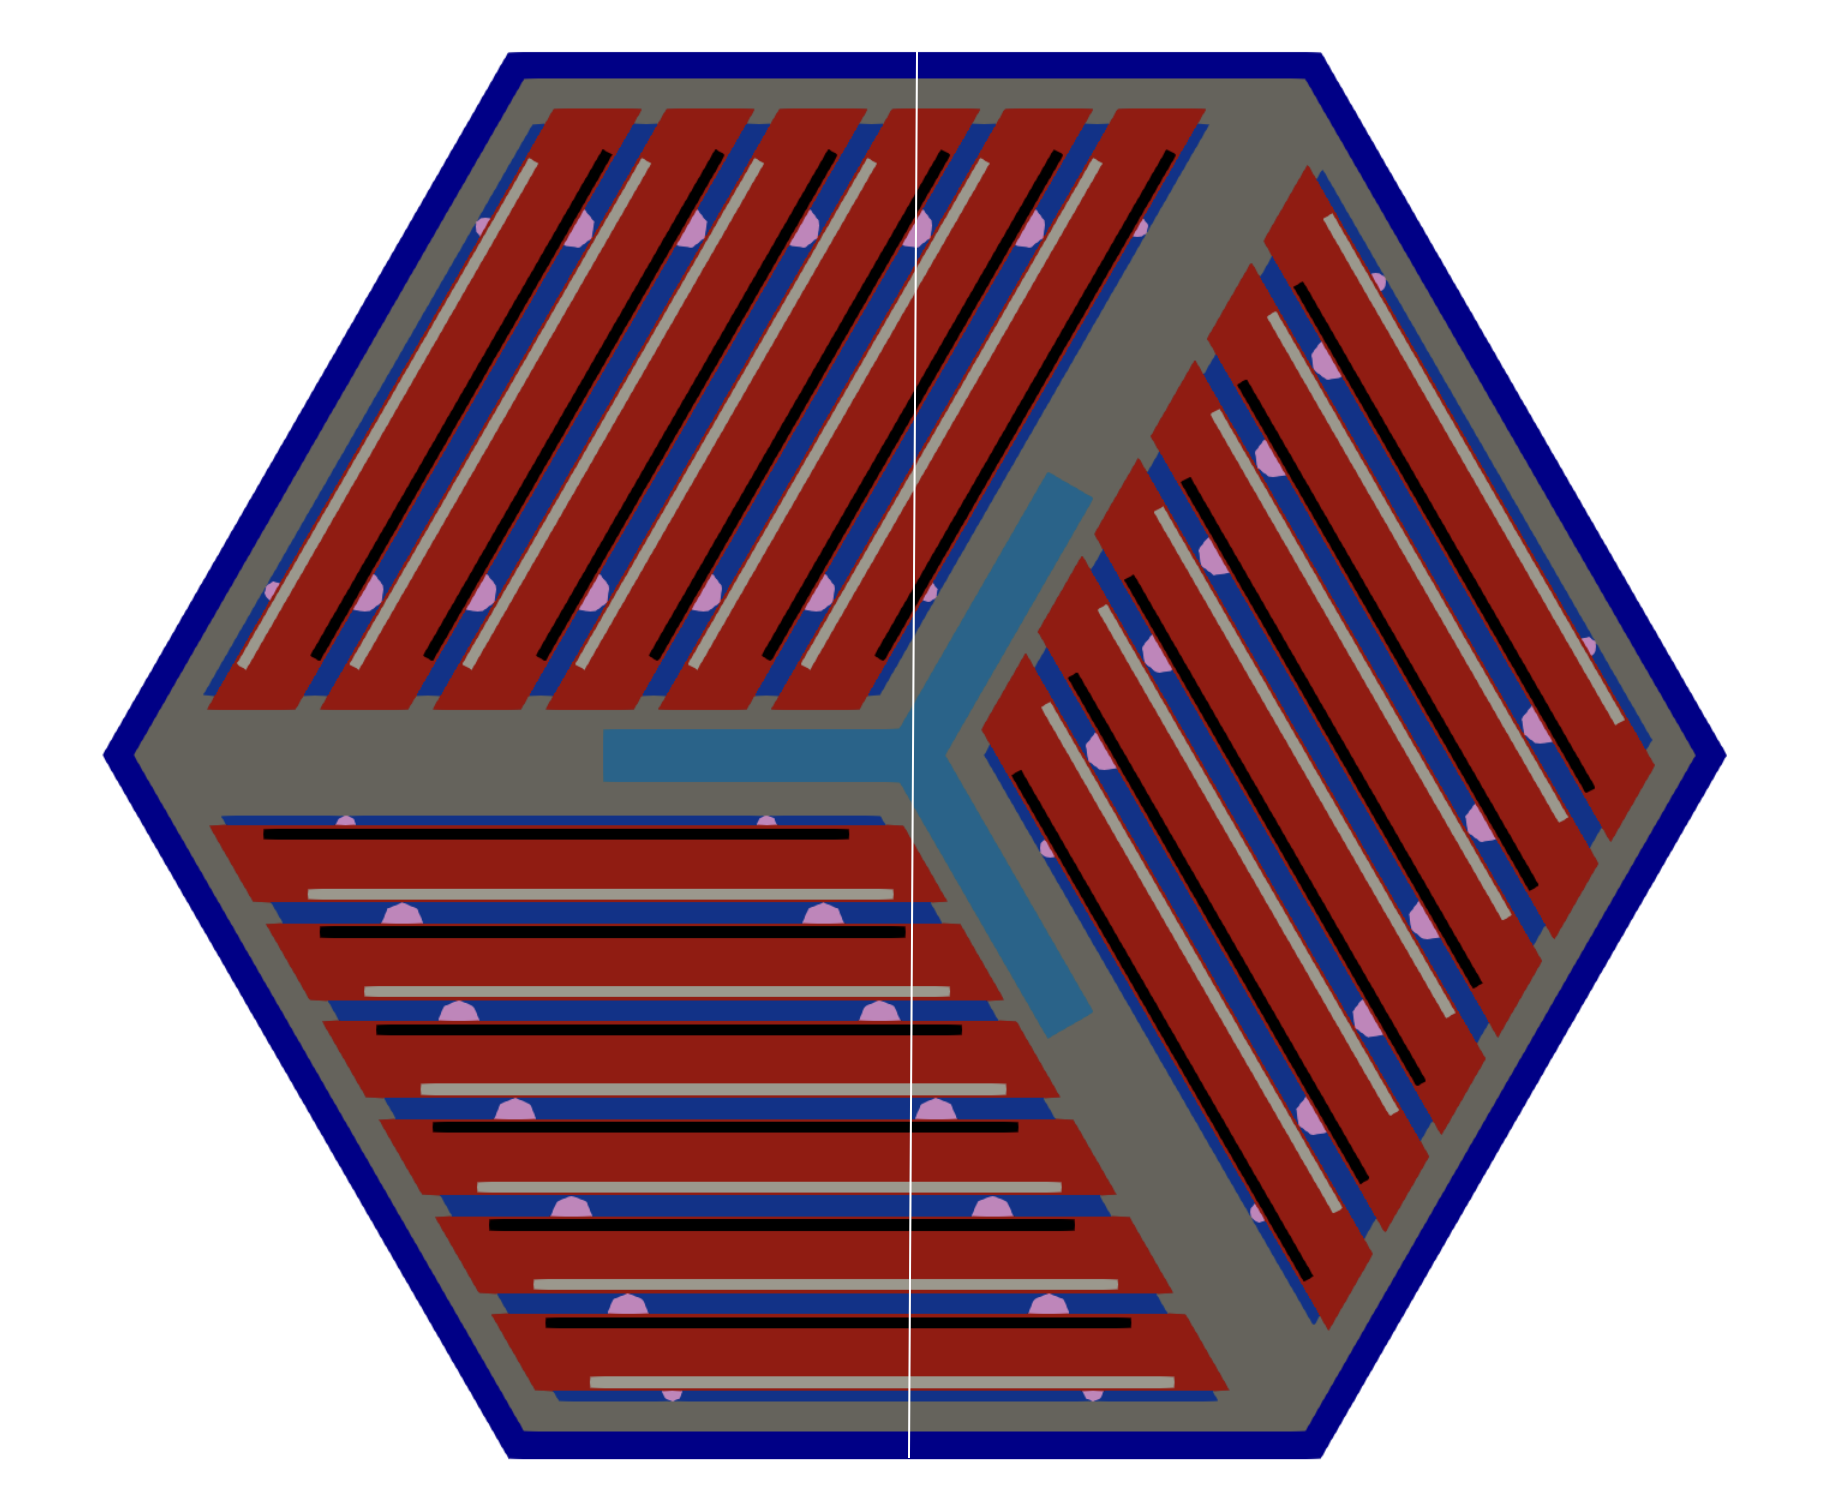
\includegraphics[width=0.5\linewidth]{../docs/figures/assembly_mg.png}
        \end{minipage}\hfill
        \begin{minipage}[c]{0.4\textwidth}
        \caption{\acrfull{AHTR} assembly spatially discretized into 61 \textit{cells} 
        for OpenMC multigroup calculation to produce group constants data for the 
        Moltres model.}
    \end{minipage}
    \end{figure}

\end{frame}